El objetivo de este trabajo practico fue adquirir destrezas sobre el funcionamiento del osciloscopio. Se pudo apreciar como distintos parámetros de la configuración del osciloscopio modifican la imagen de las señales entrantes, como fueron los ajustes de calibración de las puntas y su factor de atenuación y los distintos tipos de acoplamiento de los canales. Mejoramos en el manejo de escalas y sensibilidades para facilitar la lectura y medida de las señales además de poder modificar todos los parámetros asociados al disparo para generar un imagen clara y estable.

Como se postuló en el enunciado del trabajo practico se procedió a graficar de forma aproximada las siguientes señales:
\begin{itemize}
    \item ECG senoidal, 500Hz, amplitud 3Vpp, offset: 2V
    \item EO1 senoidal 2550Hz, amplitude 8Vp, Offset: 0V
    \item EO2 senoidal 4780Hz, amplitud 250mVpp, offset: 5V
    \item ED Senoidal 12500Hz, amplitud 12,5Vpp, offset: -10V 
\end{itemize}
Para estas señales se plantearon las siguientes configuraciones pensando en que el nivel de tensión $0V$ coincidente con la linea horizontal media del osciloscopio:
\begin{itemize}
    \item ECG: V/div=$1V$, t/div=$10 ms$, Aten.=$x1$, Acop=DC.
    \item EO1: V/div=$5V$, t/div=$1 ms$, Aten.=$x1$, Acop=DC.
    \item EO2: V/div=$2V$, t/div=$1 ms$, Aten.=$x1$, Acop=DC.
    \item ED: V/div=$2V$, t/div=$50 ms$, Aten.=$x10$, Acop=DC.
\end{itemize}

\begin{figure}[H]
    \centering
    \begin{minipage}{0.49\textwidth}
    \centering
        \begin{tikzpicture}[scale=0.5]
\def\scalT{0.01};
\def\scalV{1};
\def\offset{2};
\foreach \x in {-5,-4.8,...,4.8,5}{
    \draw[gray!40,thin,shift={(\x,0)}] (0pt,2pt) -- (0pt,-2pt);
}
\foreach \y in {-4,-3.8,...,3.8,4}{
    \draw[gray!40,thin,shift={(0,\y)}] (2pt,0pt) -- (-2pt,0pt);
}
\foreach \a [evaluate={\y=\a*2.5}] in {-1,1}{
    \draw[gray!40,thin,dotted] (-5,\y) -- (5,\y);
}

\draw[thin,gray!40] (-5,-4) grid (5,4);
\node[fill=white,text=gray!40,circle,scale=0.3] at (-5,2.5) {$100$};
\node[fill=white,text=gray!40,circle,scale=0.3] at (-5,2) {$50$};
\node[fill=white,text=gray!40,circle,scale=0.3] at (-5,-2) {$10$};
\node[fill=white,text=gray!40,circle,scale=0.3] at (-5,-2.5) {$0\%$};

\draw[black] (-6,-5) rectangle(6,5);
\draw [mblk]plot[smooth,samples=100,domain=-5:5](\x,{\scalV*(1.5*cos(deg(\x*500*\scalT))+\offset)});
\end{tikzpicture}

        \caption{Señal ECG}
    \end{minipage}
    \begin{minipage}{0.49\textwidth}
    \centering
        \begin{tikzpicture}[scale=0.5]
\def\scalT{0.001};
\def\scalV{0.2};
\def\offset{0};

\foreach \x in {-5,-4.8,...,4.8,5}{
    \draw[gray!40,thin,shift={(\x,0)}] (0pt,2pt) -- (0pt,-2pt);
}
\foreach \y in {-4,-3.8,...,3.8,4}{
    \draw[gray!40,thin,shift={(0,\y)}] (2pt,0pt) -- (-2pt,0pt);
}
\foreach \a [evaluate={\y=\a*2.5}] in {-1,1}{
    \draw[gray!40,thin,dotted] (-5,\y) -- (5,\y);
}

\draw[thin,gray!40] (-5,-4) grid (5,4);
\node[fill=white,text=gray!40,circle,scale=0.3] at (-5,2.5) {$100$};
\node[fill=white,text=gray!40,circle,scale=0.3] at (-5,2) {$50$};
\node[fill=white,text=gray!40,circle,scale=0.3] at (-5,-2) {$10$};
\node[fill=white,text=gray!40,circle,scale=0.3] at (-5,-2.5) {$0\%$};


\draw[black] (-6,-5) rectangle(6,5);

\draw [mblk]plot[smooth,samples=100,domain=-5:5](\x,{\scalV*(8*cos(deg(\x*2550*\scalT))+\offset)});
\end{tikzpicture}

        \caption{Señal EO1}
    \end{minipage}
\end{figure}
\begin{figure}[H]
    \centering
    \begin{minipage}{0.49\textwidth}
    \centering
        \begin{tikzpicture}[scale=0.5]
\def\scalT{0.001};
\def\scalV{0.5};
\def\offset{5};

\foreach \x in {-5,-4.8,...,4.8,5}{
    \draw[gray!40,thin,shift={(\x,0)}] (0pt,2pt) -- (0pt,-2pt);
}
\foreach \y in {-4,-3.8,...,3.8,4}{
    \draw[gray!40,thin,shift={(0,\y)}] (2pt,0pt) -- (-2pt,0pt);
}
\foreach \a [evaluate={\y=\a*2.5}] in {-1,1}{
    \draw[gray!40,thin,dotted] (-5,\y) -- (5,\y);
}

\draw[thin,gray!40] (-5,-4) grid (5,4);
\node[fill=white,text=gray!40,circle,scale=0.3] at (-5,2.5) {$100$};
\node[fill=white,text=gray!40,circle,scale=0.3] at (-5,2) {$50$};
\node[fill=white,text=gray!40,circle,scale=0.3] at (-5,-2) {$10$};
\node[fill=white,text=gray!40,circle,scale=0.3] at (-5,-2.5) {$0\%$};

\draw[black] (-6,-5) rectangle(6,5);

\draw [mblk]plot[smooth,samples=100,domain=-5:5](\x,{\scalV*(0.25*cos(deg(\x*(4780*\scalT)))+\offset)});
\end{tikzpicture}
        \caption{Señal EO2}
        \label{fig:EO2}
    \end{minipage}
    \begin{minipage}{0.49\textwidth}
    \centering
        \begin{tikzpicture}[scale=0.5]
\def\scalT{0.05};
\def\scalV{0.1*0.5};
\def\offset{-10};
\foreach \x in {-5,-4.8,...,4.8,5}{
    \draw[gray!40,thin,shift={(\x,0)}] (0pt,2pt) -- (0pt,-2pt);
}
\foreach \y in {-4,-3.8,...,3.8,4}{
    \draw[gray!40,thin,shift={(0,\y)}] (2pt,0pt) -- (-2pt,0pt);
}
\foreach \a [evaluate={\y=\a*2.5}] in {-1,1}{
    \draw[gray!40,thin,dotted] (-5,\y) -- (5,\y);
}

\draw[thin,gray!40] (-5,-4) grid (5,4);
\node[fill=white,text=gray!40,circle,scale=0.3] at (-5,2.5) {$100$};
\node[fill=white,text=gray!40,circle,scale=0.3] at (-5,2) {$50$};
\node[fill=white,text=gray!40,circle,scale=0.3] at (-5,-2) {$10$};
\node[fill=white,text=gray!40,circle,scale=0.3] at (-5,-2.5) {$0\%$};

\draw[black] (-6,-5) rectangle(6,5);

\clip (-5,-4) rectangle (5,4);
\draw [mblk]plot[smooth,samples=100,domain=-5:5](\x,{\scalV*(12.5*cos(deg(\x*(125*\scalT)))+\offset)});

\end{tikzpicture}
        \caption{Señal ED}
    \end{minipage}
\end{figure}
Cabe destacar que en varios casos cambiando el acoplamiento de las entradas se podría aislar el componente de alterna de las señales, para poder ser analizadas con mayor detalle si se desea, como es el caso de la señal EO2, (representada en la figura\ref{fig:EO2}). En estas configuraciones se tomo como relevante la componente de continua.
Además de lo anteriormente solicitado se nos pidió completar un formulario. Las preguntas iran asociadas a las repuestas:
\begin{itemize}
    \item [] El control de “nivel de disparo” (trigger level) que todo osciloscopio posee en el panel frontal dentro de la sección de controles de la base de tiempos sirve para:
    \begin{itemize}
        \item Ajustar el punto de inicio del barrido.
    \end{itemize}
    \item [] En el panel de controles de un osciloscopio típico, y dispuesto en la zona de controles de la base de tiempos, suele ubicarse el selector de “Fuente de disparo” cuya función es:
    \begin{itemize}
        \item Permite seleccionar entre disparo: Interno – Externo – Línea.
    \end{itemize}
    \item[] En un osciloscopio de doble trazo La presentación dual se logra mediante el empleo de una llave electrónica que actúa sobre los circuitos del eje vertical; esta llave puede trabajar en modo "Barrido alternado" (Alt.) o "Barrido troceado" (Troc.). Relacione cada uno de los modos, con las características que se listan:
    \begin{itemize}
        \item Modo "Barrido alternado" (Alt.):
        \begin{itemize}
            \item[X] En un barrido se muestra un canal, y en el siguiente el otro.
            \item[X] Se emplea cuando la velocidad de barrido es elevada.
        \end{itemize}
        \item Modo "Barrido troceado" (Troc.):
        \begin{itemize}
            \item[X] Se emplea cuando la velocidad de barrido es baja.
            \item[X] Dentro de cada ciclo de barrido se va alternado cada uno de los canales.
        \end{itemize}
    \end{itemize}
    \item[]En todos los osciloscopios de usos generales el disparo del barrido del eje X puede seleccionarse, al menos, entre “Modo automático” y “Modo normal”. En el modo normal, la base de tiempos se dispara cuando:
    \begin{itemize}
        \item El nivel de disparo está contenido entre el máximo y el mínimo de la señal de entrada.

    \end{itemize}
    \item[] En el panel de controles de todo osciloscopio, suele haber un punto de prueba (TP) donde hay disponible una señal, generada internamente, de 1KHz, con forma de onda cuadrada que según lo indicado habitualmente en los manuales se emplea para “calibra la punta de pruebas”. Dicho procedimiento se realiza:
    \begin{itemize}
        \item Con la punta en la posición X1 y es para compensar la respuesta en frecuencia.
    \end{itemize}
    \item[] La calibración de la punta, se hace observando la forma de onda cuadrada, y normalmente debe retocarse un ajuste que suele encontrarse:
    \begin{itemize}
        \item En la propia punta de pruebas, y se accede mediante un destornillador de plástico.
    \end{itemize}
    \item[] Por lo general todos los osciloscopios de doble trazo disponen, en el selector de “Modo Vertical”, de una posición denominada “ADD” (Suma). Este modo suele utilizarse juntamente con la opción “INV” (inversión) de uno de los canales Y. Cuando un osciloscopio se emplea de esta forma:
    \begin{itemize}
        \item Funciona como un instrumento de canal único y entrada diferencial.
    \end{itemize}
\end{itemize}
Por ultimo se nos pidió deducir el valor eficaz de la tensión y el ciclo de trabajo de la señal representada en la figura\ref{fig:ConcSeñ}, sabiendo que:
\begin{itemize}
    \item Eje Y= 2V/div.
    \item Base de T = 1ms/div. 
    \item La sonda de pruebas se encuentra en la posición X 10. 
    \item La forma de onda observada no tiene componente de CC.

\end{itemize}
\begin{figure}[H]
    \centering
    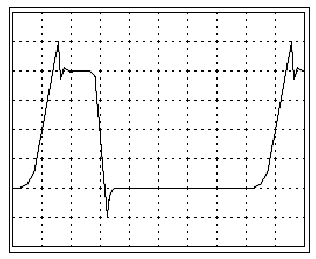
\includegraphics{Imagenes/ConcSeñ.png}
    \caption{Caption}
    \label{fig:ConcSeñ}
\end{figure}

Tomando en cuenta la configuración del osciloscopio y presuponiendo una onda cuadrada sin ciclo de trabajo negativo, el valor $V_{pp}$ de la señal va estar dado por:
\begin{equation}
    V_{pp}=10\cdot(2V\cdot divisones)
\end{equation}
En este caso la señal ocupa $4$ divisiones por lo tanto el valor $V_{pp}$ sera de:
\begin{equation}
    V_{pp}=10\cdot(2V\cdot 4)=80V
\end{equation}
El periodo para la señal es de $1ms\cdot division$, podemos apreciar que un ciclo de la señal ocupa aproximadamente $8$ divisiones de los cuales en solo $2$ la señal es activa. Entonces el ciclo de trabajo de la señal es de:
\begin{equation}
    D=\frac{T_{Actio}}{T_{total}}\cdot100\%=25\%
\end{equation}
Y pos un periodo de $T=8ms$.
Teniendo en cuenta la definición del valor eficaz y todos los datos podemos de ducir que:
\begin{equation}
\begin{aligned}
     V_{rms}=\sqrt{\frac{1}{T}\int_{0}^{T_{a}}v^2dt}\lrah &V_{rms}\thickapprox\sqrt{\frac{1}{8ms}\cdot(80^2 \cdot2ms)}\\
                                                    &V_{rms}\thickapprox\sqrt{\frac{1}{8ms}\cdot(80^2\cdot 2ms)}\\
                                                    &V_{rms}\thickapprox40V
\end{aligned}
\end{equation}
